% the periotic table from the 2002 BBC show Look Around You
% Adapted from https://texample.net/tikz/examples/periodic-table-of-chemical-elements.

\documentclass[tikz,border=15mm]{standalone}
\usepackage{fontspec}
\usepackage{xcolor}
\usetikzlibrary{backgrounds}
\setmainfont{FuturaStd.otf}

\newcommand{\LAElm}[5]{
	% \begin{tikzpicture}
		%     \drawfill (0,0) rectangle (3,3);
		% \end{tikzpicture}
	\begin{minipage}{2.4cm}
		\centering
		\begin{tikzpicture}[overlay]
			\node at (-0.9,0.2) {
				\begin{minipage}[c]{0.6cm}
					{#1 \\ #2 \\ #3}
			\end{minipage}};
			\node at (0.1, 0.2){ \huge \textbf{#4} };
			\node at (0,-0.8) {#5};
		\end{tikzpicture}
	\end{minipage}
}

\def\rowspace{0.1cm}

%define colors for Look Around You periotic table
\definecolor{textcolor}{RGB}{157,2,108}
\definecolor{pagecolor}{RGB}{231,195,178}
%elements
\definecolor{lithiumBG}{RGB}{195,155,212}
\definecolor{franceBG}{RGB}{178,168,211}
\definecolor{woodBG}{RGB}{223,154,213}
\definecolor{manBG}{RGB}{245,154,203}
\definecolor{silverBG}{RGB}{247,223,215}
\definecolor{nothingBG}{RGB}{244,155,162}
\definecolor{ironBG}{RGB}{242,167,147}
\definecolor{waxBG}{RGB}{236,196,143}
\definecolor{icalBG}{RGB}{253,231,156}
\definecolor{goldBG}{RGB}{251,200,107}
\definecolor{gooBG}{RGB}{205,220,145}
\definecolor{hiBG}{RGB}{181,223,190}
\definecolor{nitrogenBG}{RGB}{182,208,214}
\definecolor{neonBG}{RGB}{181,171,213}
\definecolor{heliumBG}{RGB}{203,156,213}
\definecolor{copperBG}{RGB}{244,152,136}
\definecolor{rhubarbBG}{RGB}{228,134,134}
\definecolor{tediumBG}{RGB}{231,197,180}
\definecolor{wineBG}{RGB}{184,139,159}
\definecolor{sulphurBG}{RGB}{253,231,156}


\begin{document}
	\pagecolor{pagecolor}% change color of page
	\color{textcolor}
	
	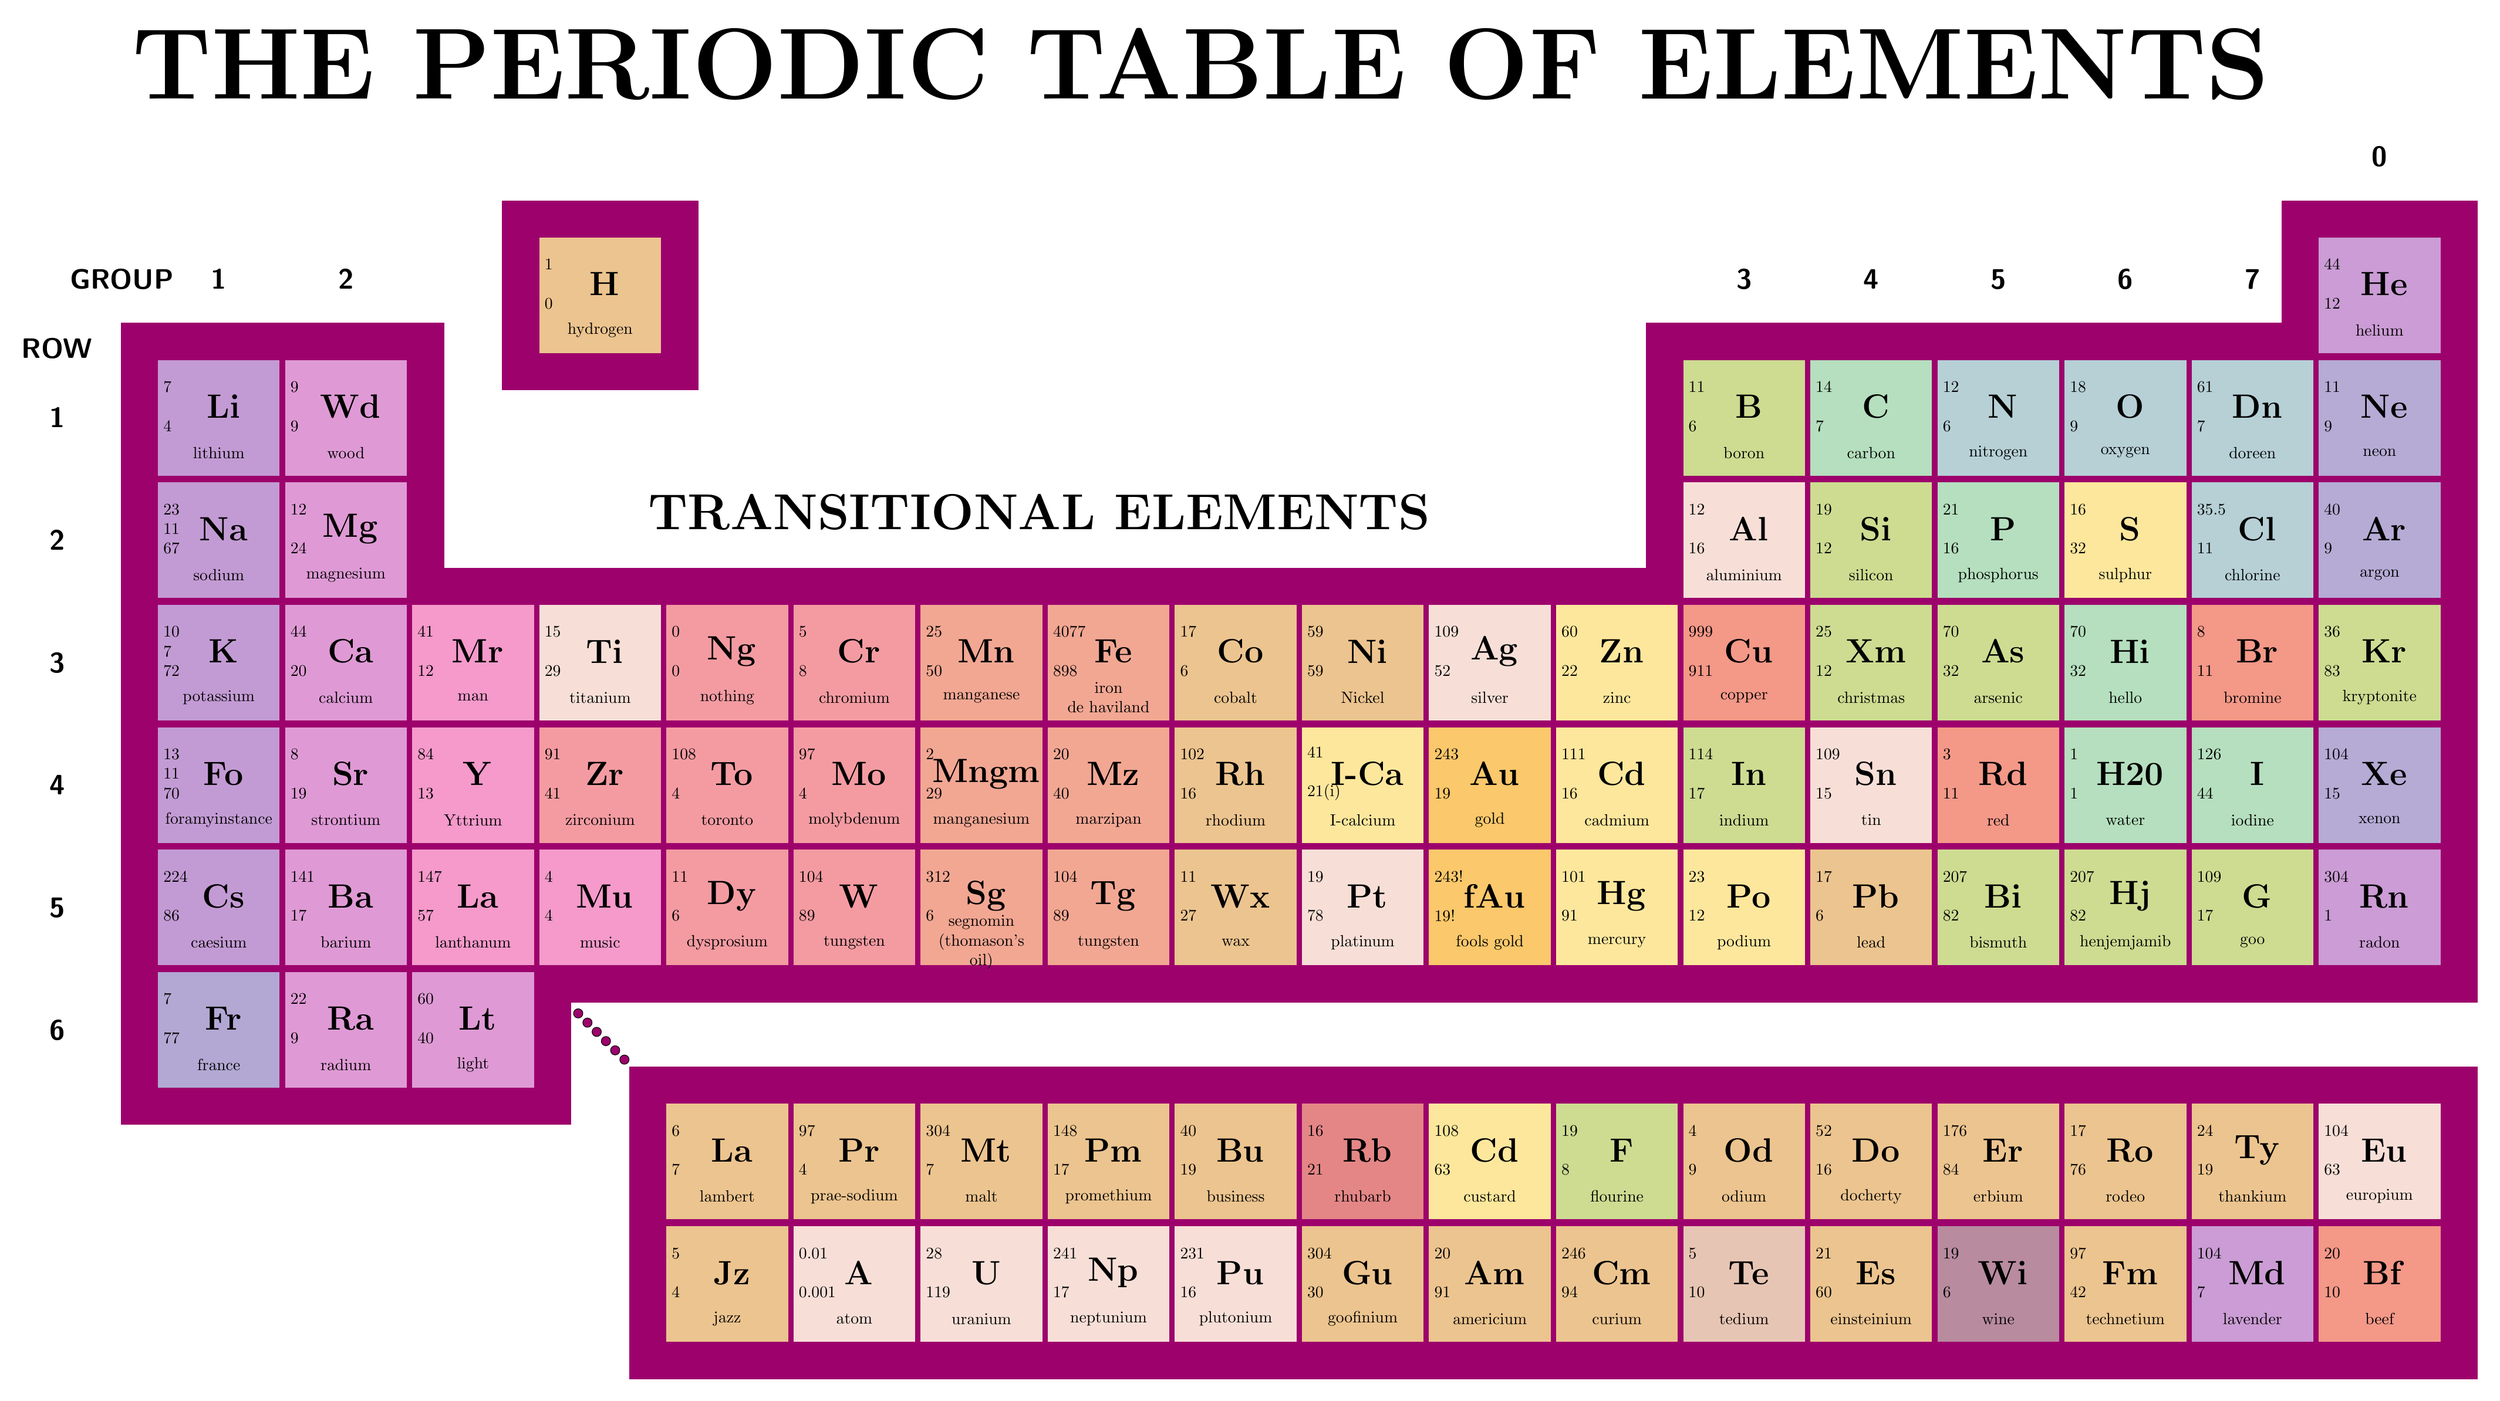
\begin{tikzpicture}
		
		% Element Styles
		\tikzstyle{Element} = [minimum width=2.5cm, minimum height=2.5cm, node distance=2.75cm]
		% to take up space in the picture
		\tikzstyle{ShadowElement} = [minimum width=2.5cm, minimum height=2.5cm, node distance=2.75cm]
		\tikzstyle{PeriodLabel} = [font={\sffamily\LARGE}, node distance=2.0cm]
		\tikzstyle{GroupLabel} = [font={\sffamily\LARGE}, minimum width=2.75cm, node distance=2.0cm]
		
		% Group 1 - IA
		\node[ShadowElement] (H) {};
		\node[right of=H,ShadowElement] (ShadowH1) {};
		\node[right of=ShadowH1,ShadowElement] (ShadowH2) {};
		\node[right of=ShadowH2,Element, fill=waxBG] (RealH) {\LAElm{1}{}{0}{H}{hydrogen}};
		
		\node[yshift=\rowspace,below of=H, Element, fill=lithiumBG] (Li) {\LAElm{7}{}{4}{Li}{lithium}};
		\node[yshift=\rowspace,below of=Li, Element, fill=lithiumBG] (Na) {\LAElm{23}{11}{67}{Na}{sodium}};
		\node[yshift=\rowspace,below of=Na, Element, fill=lithiumBG] (K) {\LAElm{10}{7}{72}{K}{potassium}};
		\node[yshift=\rowspace,below of=K, Element, fill=lithiumBG] (Rb) {\LAElm{13}{11}{70}{Fo}{foramyinstance}};
		\node[yshift=\rowspace,below of=Rb, Element, fill=lithiumBG] (Cs) {\LAElm{224}{}{86}{Cs}{caesium}};
		\node[yshift=\rowspace,below of=Cs, Element, fill=franceBG] (Fr) {\LAElm{7}{}{77}{Fr}{france}};
		
		% Group 2 - IIA
		\node[right of=Li, Element, fill=woodBG] (Be) {\LAElm{9}{}{9}{Wd}{wood}};
		\node[yshift=\rowspace,below of=Be, Element, fill=woodBG] (Mg) {\LAElm{12}{}{24}{Mg}{magnesium}};
		\node[yshift=\rowspace,below of=Mg, Element, fill=woodBG] (Ca) {\LAElm{44}{}{20}{Ca}{calcium}};
		\node[yshift=\rowspace,below of=Ca, Element, fill=woodBG] (Sr) {\LAElm{8}{}{19}{Sr}{strontium}};
		\node[yshift=\rowspace,below of=Sr, Element, fill=woodBG] (Ba) {\LAElm{141}{}{17}{Ba}{barium}};
		\node[yshift=\rowspace,below of=Ba, Element, fill=woodBG] (Ra) {\LAElm{22}{}{9}{Ra}{radium}};
		
		% Group 3 - IIIB
		\node[right of=Ca, Element, fill=manBG] (Sc) {\LAElm{41}{}{12}{Mr}{man}};
		\node[yshift=\rowspace,below of=Sc, Element, fill=manBG] (Y) {\LAElm{84}{}{13}{Y}{Yttrium}};
		\node[yshift=\rowspace,below of=Y, Element, fill=manBG] (LaLu) {\LAElm{147}{}{57}{La}{lanthanum}};
		\node[yshift=\rowspace,below of=LaLu, Element, fill=woodBG] (AcLr) {\LAElm{60}{}{40}{Lt}{light}};
		
		% Group 4 - IVB
		\node[right of=Sc, Element, fill=silverBG] (Ti)  {\LAElm{15}{}{29}{Ti}{titanium}};
		\node[yshift=\rowspace,below of=Ti, Element, fill=nothingBG] (Zr) {\LAElm{91}{}{41}{Zr}{zirconium}};
		\node[yshift=\rowspace,below of=Zr, Element, fill=manBG] (Hf)     {\LAElm{4}{}{4}{Mu}{music}};
		
		% Group 5 - VB
		\node[right of=Ti, Element, fill=nothingBG] (V)  {\LAElm{0}{}{0}{Ng}{nothing}};
		\node[yshift=\rowspace,below of=V,  Element, fill=nothingBG]  (Nb) {\LAElm{108}{}{4}{To}{toronto}};
		\node[yshift=\rowspace,below of=Nb, Element, fill=nothingBG] (Ta) {\LAElm{11}{}{6}{Dy}{dysprosium}};
		
		% Group 6 - VIB
		\node[right of=V,  Element, fill=nothingBG] (Cr) {\LAElm{5}{}{8}{Cr}{chromium}};
		\node[yshift=\rowspace,below of=Cr, Element, fill=nothingBG] (Mo) {\LAElm{97}{}{4}{Mo}{molybdenum}};
		\node[yshift=\rowspace,below of=Mo, Element, fill=nothingBG] (W)  {\LAElm{104}{}{89}{W}{tungsten}};
		
		% Group 7 - VIIB
		\node[right of=Cr, Element, fill=ironBG] (Mn) {\LAElm{25}{}{50}{Mn}{manganese}}; %TODO:
		\node[yshift=\rowspace,below of=Mn, Element, fill=ironBG] (Tc) {\LAElm{2}{}{29}{Mngm}{manganesium}};
		\node[yshift=\rowspace,below of=Tc, Element, fill=ironBG] (Re) {\LAElm{312}{}{6}{Sg}{\vbox{segnomin \\ (thomason's oil)}}};
		
		% Group 8 - VIIIB
		\node[right of=Mn, Element, fill=ironBG] (Fe) {\LAElm{4077}{}{898}{Fe}{\vbox{iron \\ de haviland}}};
		\node[yshift=\rowspace,below of=Fe, Element, fill=ironBG] (Ru) {\LAElm{20}{}{40}{Mz}{marzipan}};
		\node[yshift=\rowspace,below of=Ru, Element, fill=ironBG] (Os) {\LAElm{104}{}{89}{Tg}{tungsten}};
		
		% Group 9 - VIIIB
		\node[right of=Fe, Element, fill=waxBG] (Co) {\LAElm{17}{}{6}{Co}{cobalt}};
		\node[yshift=\rowspace,below of=Co, Element, fill=waxBG] (Rh) {\LAElm{102}{}{16}{Rh}{rhodium}};
		\node[yshift=\rowspace,below of=Rh, Element, fill=waxBG] (Ir) {\LAElm{11}{}{27}{Wx}{wax}};
		
		% Group 10 - VIIIB
		\node[right of=Co, Element, fill=waxBG] (Ni) {\LAElm{59}{}{59}{Ni}{Nickel}};
		\node[yshift=\rowspace,below of=Ni, Element, fill=icalBG] (Pd) {\LAElm{41}{}{21(i)}{I-Ca}{I-calcium}};
		\node[yshift=\rowspace,below of=Pd, Element, fill=silverBG] (Pt) {\LAElm{19}{}{78}{Pt}{platinum}};
		
		% Group 11 - IB
		\node[right of=Ni, Element, fill=silverBG] (Cu) {\LAElm{109}{}{52}{Ag}{silver}};
		\node[yshift=\rowspace,below of=Cu, Element, fill=goldBG] (Ag) {\LAElm{243}{}{19}{Au}{gold}};
		\node[yshift=\rowspace,below of=Ag, Element, fill=goldBG] (Au) {\LAElm{243!}{}{19!}{fAu}{fools gold}};
		
		% Group 12 - IIB
		\node[right of=Cu, Element, fill=icalBG] (Zn) {\LAElm{60}{}{22}{Zn}{zinc}};
		\node[yshift=\rowspace,below of=Zn, Element, fill=icalBG] (Cd) {\LAElm{111}{}{16}{Cd}{cadmium}};
		\node[yshift=\rowspace,below of=Cd, Element, fill=icalBG] (Hg) {\LAElm{101}{}{91}{Hg}{mercury}};
		
		% Group 13 - IIIA
		\node[right of=Zn, Element, fill=copperBG] (Ga)  {\LAElm{999}{}{911}{Cu}{copper}};
		\node[yshift=-\rowspace,above of=Ga, Element, fill=silverBG ] (Al)  {\LAElm{12}{}{16}{Al}{aluminium}};
		\node[yshift=-\rowspace,above of=Al, Element, fill=gooBG] (B)   {\LAElm{11}{}{6}{B}{boron}};
		\node[yshift=\rowspace,below of=Ga, Element, fill=gooBG] (In)  {\LAElm{114}{}{17}{In}{indium}};
		\node[yshift=\rowspace,below of=In, Element, fill=icalBG] (Tl)  {\LAElm{23}{}{12}{Po}{podium}};
		
		% Group 14 - IVA
		\node[right of=B,  Element, fill=hiBG] (C)   {\LAElm{14}{}{7}{C}{carbon}};
		\node[yshift=\rowspace,below of=C,  Element, fill=gooBG] (Si)  {\LAElm{19}{}{12}{Si}{silicon}};
		\node[yshift=\rowspace,below of=Si, Element, fill=gooBG] (Ge)  {\LAElm{25}{}{12}{Xm}{christmas}};
		\node[yshift=\rowspace,below of=Ge, Element, fill=silverBG] (Sn)  {\LAElm{109}{}{15}{Sn}{tin}};
		\node[yshift=\rowspace,below of=Sn, Element, fill=waxBG] (Pb)  {\LAElm{17}{}{6}{Pb}{lead}};
		
		% Group 15 - VA
		\node[right of=C,  Element, fill=nitrogenBG] (N)  {\LAElm{12}{}{6}{N}{nitrogen}};
		\node[yshift=\rowspace,below of=N,  Element,  fill=hiBG] (P)  {\LAElm{21}{}{16}{P}{phosphorus}};
		\node[yshift=\rowspace,below of=P,  Element, fill=gooBG] (As) {\LAElm{70}{}{32}{As}{arsenic}};
		\node[yshift=\rowspace,below of=As, Element, fill=copperBG] (Sb) {\LAElm{3}{}{11}{Rd}{red}};
		\node[yshift=\rowspace,below of=Sb, Element, fill=gooBG] (Bi) {\LAElm{207}{}{82}{Bi}{bismuth}};
		
		% Group 16 - VIA
		\node[right of=N, Element,fill=nitrogenBG] (O)   {\LAElm{18}{}{9}{O}{oxygen}};
		\node[yshift=\rowspace,below of=O, Element, fill=sulphurBG] (S)   {\LAElm{16}{}{32}{S}{sulphur}};
		\node[yshift=\rowspace,below of=S, Element, fill=hiBG] (Se)  {\LAElm{70}{}{32}{Hi}{hello}};
		\node[yshift=\rowspace,below of=Se,Element, fill=hiBG] (Te)  {\LAElm{1}{}{1}{H20}{water}};
		\node[yshift=\rowspace,below of=Te,Element, fill=gooBG] (Po)  {\LAElm{207}{}{82}{Hj}{henjemjamib}};
		
		% Group 17 - VIIA
		\node[right of=O,  Element,fill=nitrogenBG] (F)  {\LAElm{61}{}{7}{Dn}{doreen}};
		\node[yshift=\rowspace,below of=F,  Element,fill=nitrogenBG] (Cl) {\LAElm{35.5}{}{11}{Cl}{chlorine}};
		\node[yshift=\rowspace,below of=Cl, Element, fill=copperBG] (Br) {\LAElm{8}{}{11}{Br}{bromine}};
		\node[yshift=\rowspace,below of=Br, Element, fill=hiBG] (I)  {\LAElm{126}{}{44}{I}{iodine}};
		\node[yshift=\rowspace,below of=I,  Element, fill=gooBG] (At) {\LAElm{109}{}{17}{G}{goo}};
		
		% Group 18 - VIIIA
		\node[right of=F,  Element,fill=neonBG] (Ne) {\LAElm{11}{}{9}{Ne}{neon}};
		\node[yshift=-\rowspace,above of=Ne, Element, fill=heliumBG] (He) {\LAElm{44}{}{12}{He}{helium}};
		\node[yshift=\rowspace,below of=Ne, Element,fill=neonBG] (Ar) {\LAElm{40}{}{9}{Ar}{argon}};
		\node[yshift=\rowspace,below of=Ar, Element, fill=gooBG] (Kr) {\LAElm{36}{}{83}{Kr}{kryptonite}};
		\node[yshift=\rowspace,below of=Kr, Element,fill=neonBG] (Xe) {\LAElm{104}{}{15}{Xe}{xenon}};
		\node[yshift=\rowspace,below of=Xe, Element, fill=heliumBG] (Rn) {\LAElm{304}{}{1}{Rn}{radon}};
		
		% Period
		\node[xshift=-1.5cm,left of=Li, PeriodLabel] (Period1) {\textbf{1}};
		\node[xshift=-1.5cm,left of=Na, PeriodLabel] (Period2) {\textbf{2}};
		\node[xshift=-1.5cm,left of=K, PeriodLabel] (Period3)  {\textbf{3}};
		\node[xshift=-1.5cm,left of=Rb, PeriodLabel] (Period4) {\textbf{4}};
		\node[xshift=-1.5cm,left of=Cs, PeriodLabel] (Period5) {\textbf{5}};
		\node[xshift=-1.5cm,left of=Fr, PeriodLabel] (Period6) {\textbf{6}};
		\node[yshift=-0.5cm, above of=Period1, PeriodLabel] (Rows) {\textbf{ROW}};
		
		% Group
		\node[yshift=1cm,above of=Li, GroupLabel] (Group1) {\textbf{1}};
		\node[yshift=1cm,above of=Be, GroupLabel] (Group2) {\textbf{2}};
		\node[yshift=0cm, xshift=-0.1cm,left of=Group1, GroupLabel] (Groups) {\textbf{GROUP}};
		\node[yshift=1cm,above of=B, GroupLabel] (Group13) {\textbf{3}};
		\node[yshift=1cm,above of=C, GroupLabel] (Group14) {\textbf{4}};
		\node[yshift=1cm,above of=N, GroupLabel] (Group15) {\textbf{5}};
		\node[yshift=1cm,above of=O, GroupLabel] (Group16) {\textbf{6}};
		\node[yshift=1cm,above of=F, GroupLabel] (Group17) {\textbf{7}};
		\node[yshift=1cm,above of=He, GroupLabel] (Group18) {\textbf{0}};
		
		\node[below of= Ta, ShadowElement] (shadowlanthanide1){};
		% Lanthanide
		\node[below of=shadowlanthanide1, Element, fill=waxBG] (La) {\LAElm{6}{}{7}{La}{lambert}};
		\node[right of=La, Element, fill=waxBG] (Ce) {\LAElm{97}{}{4}{Pr}{prae-sodium}};
		\node[right of=Ce, Element, fill=waxBG] (Pr) {\LAElm{304}{}{7}{Mt}{malt}};
		\node[right of=Pr, Element, fill=waxBG] (Nd) {\LAElm{148}{}{17}{Pm}{promethium}};
		\node[right of=Nd, Element, fill=waxBG] (Pm) {\LAElm{40}{}{19}{Bu}{business}};
		\node[right of=Pm, Element, fill=rhubarbBG] (Sm) {\LAElm{16}{}{21}{Rb}{rhubarb}};
		\node[right of=Sm, Element, fill=icalBG] (Eu) {\LAElm{108}{}{63}{Cd}{custard}};
		\node[right of=Eu, Element, fill=gooBG] (Gd) {\LAElm{19}{}{8}{F}{flourine}};
		\node[right of=Gd, Element, fill=waxBG] (Tb) {\LAElm{4}{}{9}{Od}{odium}};
		\node[right of=Tb, Element, fill=waxBG] (Dy) {\LAElm{52}{}{16}{Do}{docherty}};
		\node[right of=Dy, Element, fill=waxBG] (Ho) {\LAElm{176}{}{84}{Er}{erbium}};
		\node[right of=Ho, Element, fill=waxBG] (Er) {\LAElm{17}{}{76}{Ro}{rodeo}};
		\node[right of=Er, Element, fill=waxBG] (Tm) {\LAElm{24}{}{19}{Ty}{thankium}};
		\node[right of=Tm, Element, fill=silverBG] (Yb) {\LAElm{104}{}{63}{Eu}{europium}};
		
		% Actinide
		\node[yshift=\rowspace,below of=La, Element, fill=waxBG] (Ac) {\LAElm{5}{}{4}{Jz}{jazz}};
		\node[right of=Ac, Element, fill=silverBG] (Th)  {\LAElm{0.01}{}{0.001}{A}{atom}};
		\node[right of=Th, Element, fill=silverBG] (Pa)  {\LAElm{28}{}{119}{U}{uranium}};
		\node[right of=Pa, Element, fill=silverBG] (U)   {\LAElm{241}{}{17}{Np}{neptunium}};
		\node[right of=U,  Element, fill=silverBG] (Np)  {\LAElm{231}{}{16}{Pu}{plutonium}};
		\node[right of=Np, Element, fill=waxBG] (Pu)  {\LAElm{304}{}{30}{Gu}{goofinium}};
		\node[right of=Pu, Element, fill=waxBG] (Am)  {\LAElm{20}{}{91}{Am}{americium}};
		\node[right of=Am, Element, fill=waxBG] (Cm)  {\LAElm{246}{}{94}{Cm}{curium}};
		\node[right of=Cm, Element, fill=tediumBG] (Bk)  {\LAElm{5}{}{10}{Te}{tedium}};
		\node[right of=Bk, Element, fill=waxBG] (Cf)  {\LAElm{21}{}{60}{Es}{einsteinium}};
		\node[right of=Cf, Element, fill=wineBG] (Es)  {\LAElm{19}{}{6}{Wi}{wine}};
		\node[right of=Es, Element, fill=waxBG] (Fm)  {\LAElm{97}{}{42}{Fm}{technetium}};
		\node[right of=Fm, Element, fill=heliumBG] (Md)  {\LAElm{104}{}{7}{Md}{lavender}};
		\node[right of=Md, Element, fill=copperBG] (No)  {\LAElm{20}{}{10}{Bf}{beef}};
		
		% background
		\begin{scope}[on background layer]
			\def\bordersize{0.8cm}
			%TL - top left
			%BR - bottom right
			\node[yshift=\bordersize, xshift=-\bordersize] (TL1) at (RealH.north west){}; %hydrogen
			\node[yshift=-\bordersize, xshift=\bordersize] (BR1) at (RealH.south east){};
			
			\node[yshift=\bordersize, xshift=-\bordersize] (TL2) at (Li.north west){}; %lithium to radon
			\node[yshift=-\bordersize, xshift=\bordersize] (BR2) at (Ra.south east){};
			
			\node[yshift=\bordersize, xshift=-\bordersize] (TL3) at (K.north west){}; %potassium to light
			\node[yshift=-\bordersize, xshift=\bordersize] (BR3) at (AcLr.south east){};
			
			\node[yshift=\bordersize, xshift=-\bordersize] (TL4) at (K.north west){}; %potassium to light
			\node[yshift=-\bordersize, xshift=\bordersize] (BR4) at (Rn.south east){};
			
			\node[yshift=\bordersize, xshift=-\bordersize] (TL5) at (La.north west){}; %lambert to beef
			\node[yshift=-\bordersize, xshift=\bordersize] (BR5) at (No.south east){};
			
			\node[yshift=\bordersize, xshift=-\bordersize] (TL6) at (B.north west){}; % boron to radon
			\node[yshift=-\bordersize, xshift=\bordersize] (BR6) at (Rn.south east){};
			
			\node[yshift=\bordersize, xshift=-\bordersize] (TL7) at (He.north west){}; % helium to radon
			\node[yshift=-\bordersize, xshift=\bordersize] (BR7) at (Rn.south east){};
			
			\fill[textcolor] (TL1) rectangle (BR1);
			\fill[textcolor] (TL2) rectangle (BR2);
			\fill[textcolor] (TL3) rectangle (BR3);
			\fill[textcolor] (TL4) rectangle (BR4);
			\fill[textcolor] (TL5) rectangle (BR5);
			\fill[textcolor] (TL6) rectangle (BR6);
			\fill[textcolor] (TL7) rectangle (BR7);
			
			% dots
			\draw[fill=textcolor] (TL5) + (-1mm, 1.5mm) circle (1mm);
			\draw[fill=textcolor] (TL5) + (-3mm, 3.5mm) circle (1mm);
			\draw[fill=textcolor] (TL5) + (-5mm, 5.5mm) circle (1mm);
			\draw[fill=textcolor] (TL5) + (-7mm, 7.5mm) circle (1mm);
			\draw[fill=textcolor] (TL5) + (-9mm, 9.5mm) circle (1mm);
			\draw[fill=textcolor] (TL5) + (-11mm, 11.5mm) circle (1mm);
		\end{scope}
		
		% Legend
		% \fill[AlkaliMetalFill] ($(La.north -| Fr.west) + (0,1em)$)
		% rectangle +(1em, 1em) node[right, yshift=-1.2ex]  (AlkaliMetal) {Alkali Metal};
		% \fill[AlkalineEarthMetalFill] ($(AlkaliMetal.west) - (1em,2em)$)
		% rectangle +(1em, 1em) node[right, yshift=-1.2ex] (AlkalineEarthMetal) {Alkaline Earth Metal};
		% \fill[MetalFill] ($(AlkalineEarthMetal.west) - (1em,2em)$)
		% rectangle +(1em, 1em) node[right, yshift=-1.2ex] (Metal) {Metal};
		% \fill[MetalloidFill] ($(Metal.west) - (1em,2em)$)
		% rectangle +(1em, 1em) node[right, yshift=-1.2ex] (Metalloid) {Metalloid};
		% \fill[NonmetalFill] ($(Metalloid.west) - (1em,2em)$)
		% rectangle +(1em, 1em) node[right, yshift=-1.2ex] (Non-metal) {Non-metal};
		% \fill[HalogenFill] ($(Non-metal.west) - (1em,2em)$)
		% rectangle +(1em, 1em) node[right, yshift=-1.2ex] (Halogen) {Halogen};
		% \fill[NobleGasFill] ($(Halogen.west) - (1em,2em)$)
		% rectangle +(1em, 1em) node[right, yshift=-1.2ex] (NobleGas) {Noble Gas};
		% \fill[ElementFill] ($(NobleGas.west) - (1em,2em)$) rectangle +(1em, 1em) node[right, yshift=-1.2ex] (Lanthanide/Actinide) {Lanthanide/Actinide};
		%
		% \node at (Ac -| Fr) [draw, Element, fill=white] (legend) {\NaturalElem{Z}{mass}{\LARGE Symbol}{Name}};
		% \node[align=left] at (Ac -| Ra) {black: natural\\\color{gray}gray: man-made};
		
		% Diagram Title
		\node at (H.west -| Fe.north) [yshift=5cm, xshift=2cm, scale=2.5, font={\Huge\bfseries}]
		{THE PERIODIC TABLE OF ELEMENTS};
		\node at (Fe.north) [yshift=2cm, xshift=-1.5cm, scale=1.5, font={\huge\bfseries}]{TRANSITIONAL ELEMENTS};
		
		
	\end{tikzpicture}
	
\end{document}
